% =============================================================================
% Polarity-Routed Cascade Diffusion for Crop Waste Prediction
% Target: Computers and Electronics in Agriculture (Elsevier)
% =============================================================================
\documentclass[preprint,12pt,authoryear]{elsarticle}

% --- Mathematics ---
\usepackage{amsmath,amssymb,amsthm,mathtools}
\usepackage{bm}

% --- Graphics and tables ---
\usepackage{graphicx}
\usepackage{booktabs}
\usepackage{multirow}
\usepackage{array}
\usepackage{float}
\usepackage{subcaption}
\usepackage{tabularx}

% --- Cross-referencing ---
\usepackage[colorlinks=true,citecolor=blue,linkcolor=blue,urlcolor=blue]{hyperref}

% --- Miscellaneous ---
\usepackage{xcolor}
\usepackage{enumitem}
\usepackage{microtype}
\usepackage{lineno}

% --- Custom commands ---
\newcommand{\Gcommodity}{\mathcal{G}_{\text{comm}}}
\newcommand{\Ggeo}{\mathcal{G}_{\text{geo}}}
\newcommand{\R}{\mathbb{R}}
\DeclareMathOperator{\softmax}{softmax}

% --- Theorem environments ---
\newtheorem{proposition}{Proposition}
\newtheorem{corollary}{Corollary}
\newtheorem{hypothesis}{Hypothesis}

\journal{Computers and Electronics in Agriculture}

\begin{document}

\begin{frontmatter}

\title{Polarity-Routed Cascade Diffusion for Crop Waste Prediction\\in U.S.\ Agricultural Economic Networks}

\author[inst1]{Keshav Krishnan}
\ead{keshav@cascrop.org}

\affiliation[inst1]{organization={Independent Researcher}}

% =============================================================================
% ABSTRACT
% =============================================================================
\begin{abstract}
Crop waste costs U.S.\ agriculture roughly \$19 billion annually in insurance indemnities alone. Existing prediction models treat counties as independent units, ignoring the economic contagion that propagates through commodity supply chains. We propose polarity-routed cascade diffusion, a feature engineering framework where negative price shocks propagate through commodity-specific supply chain graphs and positive signals follow geographic proximity networks. The core insight: oversupply cascades spread along commodity channels (a corn glut in Iowa depresses corn prices in Ohio), while demand-driven gains diffuse through regional geography. We validate on 638,622 USDA records spanning 2,130 U.S.\ counties and three major commodities (corn, soybeans, wheat) from 2015 to 2025. On a random split, the polarity-routed model achieves 0.935 AUC-ROC---a significant improvement over the local-only baseline at 0.917 ($p < 0.001$) and over symmetric diffusion at 0.934 ($p = 0.0002$). The entire framework uses a 13,703-parameter multilayer perceptron; novelty lies in the features, not the classifier. A temporal split (train 2015--2019, test 2022--2024) reveals that the local-only model (0.910 AUC-ROC) dominates all graph-augmented variants, exposing the non-stationarity of economic contagion patterns across time. We ground these empirical findings in a formal economic model showing that waste contagion arises from market connectivity and that positive and negative supply shocks have provably asymmetric effects on neighboring regions. These results carry practical implications for crop insurance pricing and county-level early warning systems.
\end{abstract}

\begin{keyword}
crop waste prediction \sep graph diffusion \sep economic contagion \sep polarity routing \sep agricultural networks \sep feature engineering
\end{keyword}

\end{frontmatter}

\linenumbers

% =============================================================================
% GRAPHICAL ABSTRACT
% =============================================================================
\begin{figure}[t]
    \centering
    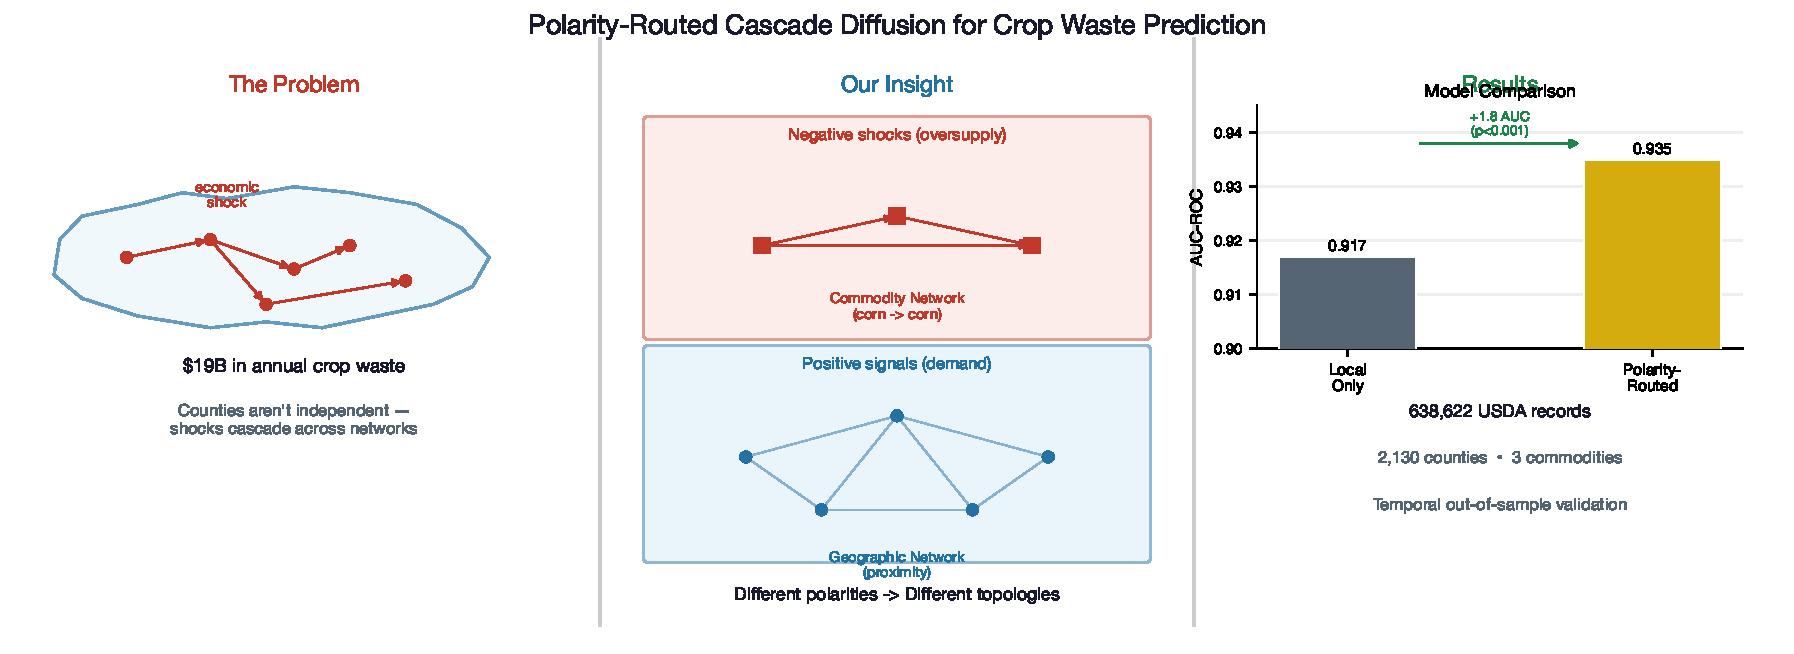
\includegraphics[width=\textwidth]{figures/fig0_graphical_abstract}
    \caption*{\textbf{Graphical Abstract.} Crop waste cascades through agricultural economic networks. Negative price shocks propagate along commodity-specific supply chains, while positive signals follow geographic proximity. Routing these signals through different graph topologies---polarity-routed cascade diffusion---improves crop waste prediction to 0.935 AUC-ROC on 638,622 USDA records across 2,130 U.S.\ counties.}
\end{figure}

% =============================================================================
% 1. INTRODUCTION
% =============================================================================
\section{Introduction}
\label{sec:introduction}

In 2023, the USDA Risk Management Agency disbursed over \$19 billion in crop insurance indemnities \citep{rma2024summary}. Much of that money covered crops that grew just fine---then went to waste. Fields were abandoned because market prices fell below harvesting costs. Standing corn was plowed under because a bumper harvest three states away flooded the commodity market. Globally, food loss and waste constitute a trillion-dollar drag on agricultural economies \citep{fao2019food}.

These waste events are not independent. They cascade.

When Iowa produces record corn yields, the resulting supply glut depresses prices across the Midwest. Farmers in Illinois, Indiana, and Ohio---whose crops may be perfectly healthy---face the cold arithmetic of harvesting at a loss. Some choose to abandon. This mechanism mirrors financial contagion: a shock at one node propagates through network connections to cause failures at distant nodes \citep{acemoglu2015systemic,elliott2014financial}. The analogy runs deep. Agricultural markets share the structural properties that produce cascading failures in financial networks: high interconnectedness through commodity exchanges, threshold effects where small price changes tip harvesting decisions, and asymmetric responses to positive versus negative shocks \citep{battiston2012debtrank}.

Yet every crop prediction model treats counties as islands. Hundreds of papers use satellite imagery, weather data, and soil characteristics to forecast yields for individual regions \citep{vanklompenburg2020crop,kang2020comparative,basso2019seasonal,lobell2011climate}. These models predict the wrong thing. They predict how much a crop \emph{will produce}, not whether it \emph{will be wasted}. High-yield crops go entirely to waste when prices crash. Low-yield crops get fully utilized when prices surge. Waste depends on biology \emph{and} economics---and the economics propagate across regions.

Graph neural networks offer a natural framework for modeling inter-regional dependencies \citep{kipf2017gcn,velickovic2018gat}. However, they bring significant complexity: end-to-end training over graph structures, poor scalability to large networks, and reduced interpretability. Recent work on simplified graph convolutions \citep{wu2019sgc,rossi2020sign} showed that pre-computing graph features---propagating node signals through the adjacency matrix before training---can match GNN performance at a fraction of the cost.

We build on this insight with a critical domain-specific innovation: \textbf{polarity-routed diffusion}. Standard graph diffusion propagates all signals through a single topology. We argue---and demonstrate---that economic shocks in agriculture are \emph{polarity-dependent}. Negative price shocks (from oversupply) propagate through commodity-specific networks: a corn glut in Iowa affects other corn-producing counties. Positive price signals (from undersupply or demand spikes) propagate through geographic proximity: when prices rise regionally, nearby counties benefit regardless of commodity mix. Routing signals through different graph topologies based on their polarity captures this fundamental asymmetry.

We formalize this intuition with a simple economic model (Section~\ref{sec:economic_model}) that yields three testable predictions. Supply shocks in one county depress prices---and increase waste risk---in market-connected counties. This contagion is provably asymmetric: positive and negative shocks follow different propagation channels. These theoretical results map directly onto our feature engineering choices.

Our contributions:

\begin{enumerate}[leftmargin=*]
    \item \textbf{Polarity-routed cascade diffusion.} We introduce a feature engineering framework where negative and positive economic signals propagate through different graph topologies (commodity-specific vs.\ geographic) at multiple hops. To our knowledge, this is the first work to route graph signals through different topologies based on shock polarity.

    \item \textbf{Formal economic model of waste contagion.} We derive propositions showing that waste contagion arises from market connectivity and that positive and negative supply shocks have provably asymmetric effects. These results justify the polarity routing mechanism from first principles.

    \item \textbf{Cascade decay signatures and cross-commodity interference.} We introduce hop-by-hop attenuation ratios that capture shock persistence and cross-commodity features that measure interference from other commodities grown in the same county.

    \item \textbf{Large-scale empirical validation.} We evaluate on 638,622 samples across 2,130 U.S.\ counties and three commodities (2015--2025), with both random and temporal splits. The temporal split reveals important non-stationarity in spatial economic patterns.

    \item \textbf{Computational efficiency by design.} The entire framework---pre-computed features fed into a 13,703-parameter MLP---trains in under a minute. The novelty is in the features, not the classifier.
\end{enumerate}


% =============================================================================
% 2. ECONOMIC MODEL
% =============================================================================
\section{Economic Model of Crop Waste Contagion}
\label{sec:economic_model}

Why does a bumper harvest in one county cause crop waste hundreds of miles away?
Standard agronomic models treat waste as a local phenomenon---drought, pest damage, frost---and ignore the market channel entirely.
We formalize the economic mechanism that propagates waste across regions, derive testable predictions, and show how these predictions map to specific feature engineering choices in our cascade diffusion framework.

\subsection{Model Setup}
\label{sec:model_setup}

Consider $N$ agricultural regions (counties) indexed by $i = 1, \ldots, N$.
Each region $i$ grows a commodity with production quantity $q_i$, determined by biophysical conditions (weather, soil, planted acreage), and faces a harvesting cost $c_i > 0$ encompassing labor, fuel, and equipment.
The farmer in region $i$ observes a local market price $p_i$ and harvests if and only if revenue exceeds cost:
\begin{equation}
\label{eq:harvest_condition}
p_i \cdot q_i > c_i.
\end{equation}
When this condition fails, the standing crop is abandoned---left unharvested and wasted.

The local price depends on aggregate regional supply through a linear inverse demand system:
\begin{equation}
\label{eq:price}
p_i = P^{\mathrm{global}} - \sum_{j=1}^{N} \beta_{ij} \, q_j,
\end{equation}
where $P^{\mathrm{global}} > 0$ is the national or world reference price and $\beta_{ij} \geq 0$ captures \emph{market connectivity} between regions $i$ and $j$.

\paragraph{Interpretation of $\beta_{ij}$.}
The coefficient $\beta_{ij}$ encodes how strongly production in region $j$ depresses the price received by farmers in region $i$.
Four properties govern its structure:
\begin{enumerate}[label=(\roman*)]
    \item $\beta_{ij} > 0$ if and only if regions $i$ and $j$ compete in the same downstream market (shared processors, packers, or distribution channels).
    \item $\beta_{ij}$ increases with geographic proximity, since transportation costs determine which buyers are accessible.
    \item $\beta_{ij}$ increases with commodity similarity---two adjacent corn-producing counties interact more strongly than a corn county and a soybean county.
    \item $\beta_{ij} \approx 0$ for distant or market-disconnected regions.
\end{enumerate}
These properties make the matrix $\mathbf{B} = [\beta_{ij}]$ sparse, spatially structured, and commodity-dependent---precisely the adjacency structure our graph model learns from data.

\paragraph{Waste probability.}
Define the \emph{profit margin} for region $i$ as
\begin{equation}
\label{eq:margin}
\pi_i \;=\; p_i \cdot q_i - c_i \;=\; \left(P^{\mathrm{global}} - \sum_{j} \beta_{ij}\, q_j \right) q_i \;-\; c_i.
\end{equation}
Region $i$ wastes its crop whenever $\pi_i \leq 0$.
In a stochastic setting where $q_j$ is drawn from a distribution $F_j$ (reflecting weather uncertainty), the waste probability is
\begin{equation}
\label{eq:waste_prob}
\Pr(\text{waste}_i) = \Pr\!\left(\pi_i \leq 0\right) = \Pr\!\left(\sum_{j} \beta_{ij}\, q_j \geq P^{\mathrm{global}} - \frac{c_i}{q_i}\right).
\end{equation}

\subsection{Waste Contagion}

\begin{proposition}[Waste Contagion]
\label{prop:contagion}
Let region $j$ experience a positive supply shock: $q_j$ increases to $q_j + \Delta q_j$ with $\Delta q_j > 0$, while all other quantities $\{q_k\}_{k \neq j}$ remain unchanged.
If $\beta_{ij} > 0$, then the waste probability in region $i$ strictly increases, even when region $i$'s own biophysical conditions are unchanged.
\end{proposition}

\begin{proof}
From Equation~\eqref{eq:price}, the price in region $i$ after the shock is
\[
p_i' = P^{\mathrm{global}} - \sum_{k \neq j} \beta_{ik}\, q_k - \beta_{ij}(q_j + \Delta q_j) = p_i - \beta_{ij}\, \Delta q_j.
\]
Since $\beta_{ij} > 0$ and $\Delta q_j > 0$, we have $p_i' < p_i$.
The post-shock profit margin becomes
\[
\pi_i' = p_i' \cdot q_i - c_i = \pi_i - \beta_{ij}\, \Delta q_j \cdot q_i < \pi_i.
\]
Because $q_i > 0$ (region $i$ has a standing crop), the margin drops by the strictly positive quantity $\beta_{ij}\, \Delta q_j \, q_i$.
Hence $\Pr(\pi_i' \leq 0) > \Pr(\pi_i \leq 0)$, and the waste probability in region $i$ strictly increases.
\end{proof}

Proposition~\ref{prop:contagion} captures the central paradox of crop waste: good weather in one county can destroy value in another.
The mechanism is purely economic---no pathogen spreads, no pest migrates.
A bumper harvest floods shared markets, crashes the local price, and pushes marginal farmers below their break-even threshold.
The strength of this contagion depends entirely on $\beta_{ij}$, the market connectivity \citep{acemoglu2015systemic}.

\begin{corollary}[Asymmetric Propagation]
\label{cor:asymmetry}
Positive and negative supply shocks in region $j$ have asymmetric effects on waste in region $i$:
\begin{enumerate}[label=(\alph*)]
    \item \textbf{Bumper harvest} ($\Delta q_j > 0$): $p_i$ falls by $\beta_{ij}\, \Delta q_j$, \emph{increasing} waste probability in $i$.
    \item \textbf{Crop failure} ($\Delta q_j < 0$): $p_i$ rises by $\beta_{ij}\, |\Delta q_j|$, \emph{decreasing} waste probability in $i$.
\end{enumerate}
Consequently, the effect of neighbor shocks on waste risk is directionally asymmetric: positive supply shocks are harmful and negative supply shocks are beneficial to region $i$'s harvest viability.
\end{corollary}

The proof follows immediately from Proposition~\ref{prop:contagion} by substituting $\Delta q_j < 0$.
This asymmetry has a direct implication for feature engineering: a predictive model must condition on the \emph{sign} of neighbor shocks, not merely their magnitude.
Symmetric diffusion---treating $+\Delta q_j$ and $-\Delta q_j$ identically---discards the directional information that distinguishes waste-inducing from waste-relieving shocks.
This motivates the polarity routing in our cascade diffusion framework.

\subsection{Testable Hypotheses}
\label{sec:hypotheses}

The model generates three predictions that map directly to our ablation experiments.

\begin{hypothesis}[Graph Structure Improves Prediction]
\label{hyp:graph}
Because waste contagion propagates through the connectivity matrix $\mathbf{B}$, models that capture inter-regional dependencies will outperform models that treat each region independently.
\end{hypothesis}

\noindent\textit{Test.}\; Compare polarity-routed (which includes graph-derived features) against local-only (which has no inter-regional information).

\begin{hypothesis}[Economic Edges Outperform Geographic Proximity]
\label{hyp:edges}
Since $\beta_{ij}$ depends on market structure and commodity similarity---not geographic distance alone---edges derived from commodity-specific connectivity will carry more predictive signal than a single undirected geographic graph.
\end{hypothesis}

\noindent\textit{Test.}\; Compare polarity-routed (which uses commodity-specific graphs for negative shocks) against cascade direct (which uses a single combined graph).

\begin{hypothesis}[Directional Conditioning Captures Asymmetry]
\label{hyp:asymmetry}
By Corollary~\ref{cor:asymmetry}, positive and negative neighbor shocks have opposite effects on waste risk.
Models that condition on shock direction will outperform symmetric alternatives.
\end{hypothesis}

\noindent\textit{Test.}\; Compare polarity-routed against symmetric diffusion, which propagates both polarities through the same topology.

\paragraph{From theory to features.}
These three hypotheses jointly motivate every key design choice.
Hypothesis~\ref{hyp:graph} justifies graph-derived features over local-only models.
Hypothesis~\ref{hyp:edges} drives our commodity-specific graph construction.
Hypothesis~\ref{hyp:asymmetry} motivates the polarity routing mechanism that separates surplus and deficit signals during neighborhood aggregation.
Section~\ref{sec:methods} details how we translate each theoretical requirement into a concrete feature engineering step.


% =============================================================================
% 3. RELATED WORK
% =============================================================================
\section{Related Work}
\label{sec:related_work}

The economic model establishes \emph{what} should propagate (signed supply shocks) and \emph{through what} (market connectivity). We now survey the computational tools available for implementing these ideas, identifying where existing methods fall short and where our contribution fits.

\subsection{Crop Yield and Loss Prediction}

Machine learning for crop yield prediction has matured rapidly \citep{vanklompenburg2020crop}. Deep Gaussian processes \citep{you2017deep}, CNN-RNN hybrids \citep{khaki2020cnn}, and attention-based architectures \citep{wang2020winter} have all pushed accuracy on county-level yield forecasting. Satellite-derived vegetation indices remain the dominant input \citep{huete2002overview,wolanin2020estimating}. More recently, \citet{peng2025multitask} demonstrated multi-task learning across multiple commodities, and \citet{ding2022integrating} integrated economic indicators alongside remote sensing features for crop classification.

Crop insurance modeling represents a parallel line of work. \citet{goodwin2004premium} examined premium rate determination in the Federal Crop Insurance Program, while \citet{yu2018assessing} applied machine learning to assess loss experience and premium adequacy across U.S.\ counties.

A consistent gap runs through all of this work: counties are treated as independent observations. None of these models capture the inter-regional economic dependencies that drive waste cascades. Moreover, most predict yield rather than waste---a fundamentally different target. A 200-bushel-per-acre corn harvest can be entirely wasted if the price falls below harvesting cost. Yield and waste require separate modeling paradigms.

\subsection{Graph-Based Methods in Agriculture}

Graph neural networks (GNNs) have seen growing application in spatial agricultural modeling. \citet{fan2022gnn_crop} used graph convolutions \citep{kipf2017gcn} to capture spatial dependencies in crop yield prediction across Chinese counties. Graph attention networks \citep{velickovic2018gat} learn which spatial connections matter most, while GraphSAGE \citep{hamilton2017graphsage} and GIN \citep{xu2019powerful} extended graph learning to inductive settings. Supply chain disruption prediction using GNNs \citep{kosasih2022graph,brintrup2020supply} has been explored in industrial contexts, and the framework translates naturally to agricultural commodity networks.

However, full GNNs impose computational and practical burdens: end-to-end training on graph structures, sensitivity to graph construction, and limited scalability. For the 2,130-county network we study, the overhead is difficult to justify when simpler approaches can capture the same structural signal.

\subsection{Economic Contagion in Networks}

The study of contagion in financial networks \citep{acemoglu2015systemic,elliott2014financial,gai2010contagion} established that shocks propagate through economic linkages in ways that depend on network topology and shock characteristics. \citet{battiston2012debtrank} introduced DebtRank to quantify systemic risk from cascading defaults. \citet{glasserman2016contagion} surveyed contagion mechanisms, while \citet{jackson2014networks} situated network effects within broader economic behavior.

The core insight from this literature---that shock propagation is directional and asymmetric---motivates our polarity routing. Agricultural commodity markets exhibit nonlinear price transmission \citep{serra2011nonlinear} and complex mean-variance dynamics \citep{harri2011mean}. Spatial econometric methods \citep{lesage2009introduction,anselin2003spatial} have long modeled spatial dependencies in economic data, but these approaches assume linear spatial lag structures and cannot capture polarity-dependent routing. Despite the strong theoretical foundation, no prior work has applied polarity-dependent network diffusion to agricultural prediction.

\subsection{Pre-Computed Graph Features}

\citet{wu2019sgc} showed that removing nonlinearities between GCN layers---collapsing $K$ layers of graph convolution into a single matrix power $\tilde{A}^K X$---achieves competitive performance at a fraction of the cost. SIGN \citep{rossi2020sign} extended this by concatenating features diffused at multiple hops ($\tilde{A}^0 X, \tilde{A}^1 X, \ldots, \tilde{A}^K X$) and feeding them into a standard MLP. \citet{chen2020simple} demonstrated that deep graph convolutions with careful normalization match more complex architectures.

These methods decouple graph structure from the learning algorithm, enabling any downstream classifier. Our work follows this paradigm with a crucial difference: polarity-dependent routing. Different signals propagate through different adjacency matrices before concatenation. Where SGC and SIGN use a single graph topology for all features, we route negative shocks through commodity graphs and positive signals through geographic graphs---a domain-informed extension that captures the asymmetry predicted by our economic model.


% =============================================================================
% 4. MATERIALS AND METHODS
% =============================================================================
\section{Materials and Methods}
\label{sec:methods}

The theoretical framework from Section~\ref{sec:economic_model} tells us that waste contagion depends on market connectivity, shock polarity, and commodity similarity. The literature review in Section~\ref{sec:related_work} reveals that no existing method captures all three. We now describe how polarity-routed cascade diffusion translates these requirements into a concrete, computationally efficient pipeline.

\subsection{Dataset Description}
\label{sec:data}

We construct a dataset of 638,622 county-commodity-month observations spanning 2015--2025 across the continental United States. Table~\ref{tab:dataset} summarizes the data sources and coverage. Figure~\ref{fig:study_area} shows the geographic distribution of counties in the study.

\begin{table}[t]
\centering
\caption{Dataset summary: sources, coverage, and key statistics.}
\label{tab:dataset}
\begin{tabular}{@{}ll@{}}
\toprule
\textbf{Attribute} & \textbf{Value} \\
\midrule
Observations & 638,622 county-commodity-month records \\
Counties & 2,130 (continental U.S.) \\
Commodities & Corn, soybeans, wheat \\
Temporal range & January 2015 -- December 2025 \\
Temporal resolution & Monthly \\
Waste rate & 18\% of observations \\
Label source & USDA RMA cause-of-loss database \citep{rma2024summary} \\
Biophysical sources & USDA NASS county production data, \\
 & NOAA Climate Division monthly summaries \citep{noaa2024} \\
Economic sources & USDA ERS \citep{usdaers2024}, BLS Producer Price Indices \\
Graph sources & U.S.\ Census Bureau county adjacency \\
\bottomrule
\end{tabular}
\end{table}

\begin{figure}[t]
    \centering
    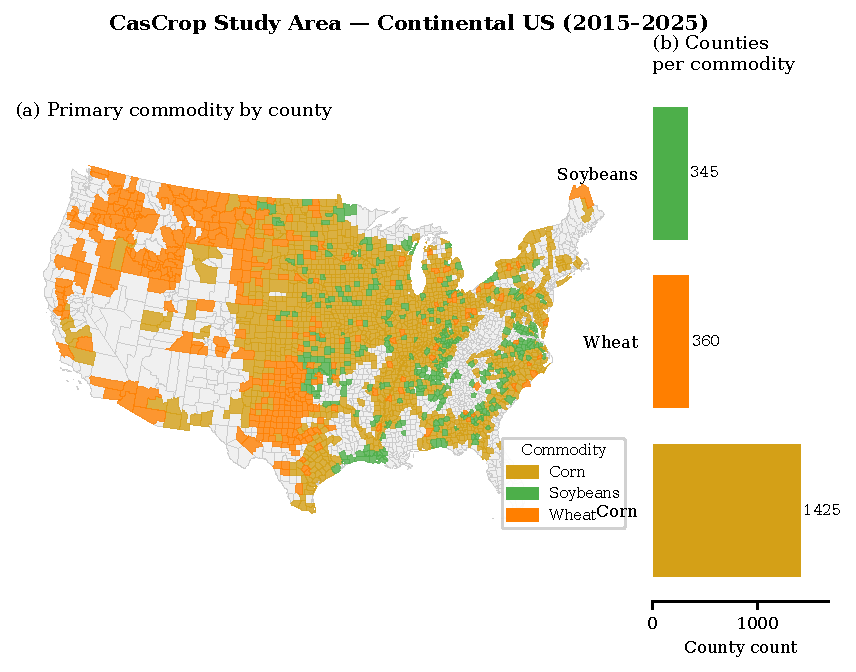
\includegraphics[width=\textwidth]{figures/fig2_study_area}
    \caption{Study area: 2,130 U.S.\ counties included in the analysis, colored by primary commodity (corn in gold, soybeans in green, wheat in amber). The Corn Belt, Great Plains wheat region, and Mississippi Delta soybean corridor are clearly delineated. Inset shows county counts by commodity.}
    \label{fig:study_area}
\end{figure}

The dataset covers three major commodity groups---corn, soybeans, and wheat---with monthly temporal resolution that captures both growing-season dynamics and off-season market movements. We construct a binary waste label from USDA RMA cause-of-loss records: an observation is labeled positive when the county-commodity-month indemnity exceeds a threshold calibrated to balance noise reduction against label coverage. The overall waste rate is 18\%.

\subsection{Feature Engineering}
\label{sec:features}

Each observation is described by 50 features organized into four groups (Table~\ref{tab:feature_groups}).

\begin{table}[t]
\centering
\caption{Feature groups comprising the complete 50-dimensional input vector.}
\label{tab:feature_groups}
\begin{tabular}{@{}p{3.2cm}rp{8cm}@{}}
\toprule
\textbf{Feature Group} & \textbf{Count} & \textbf{Features} \\
\midrule
Biophysical & 19 & yield value, area planted, area harvested, production, NASS waste proxy, max temperature, min temperature, mean temperature, precipitation, Palmer Drought Severity Index, cooling degree days, heating degree days, temperature range, growing degree day proxy, latitude, longitude, land area, month sine, month cosine \\[4pt]
Economic & 8 & commodity price, 1-month price change, 3-month price mean, 3-month price std, 3-month price volatility, year-over-year price change, county production share, county shock index \\[4pt]
Historical & 3 & historical waste rate, historical average indemnity, historical loss count \\[4pt]
Cascade (graph-derived) & 20 & 6 polarity-routed diffusion (3 hops $\times$ 2 polarities), 4 decay signatures (2 transitions $\times$ 2 polarities), 2 cross-commodity interference, 8 neighborhood-diffused \\
\midrule
\textbf{Total} & \textbf{50} & \\
\bottomrule
\end{tabular}
\end{table}

\subsubsection{Biophysical Features (19)}

We derive 19 biophysical features from USDA NASS county-level production data and NOAA climate division records. Production variables include yield value, area planted, area harvested, total production, and a NASS-derived waste proxy (ratio of planted-to-harvested area). Weather variables---maximum, minimum, and mean temperature, precipitation, Palmer Drought Severity Index (PDSI), cooling and heating degree days, temperature range, and a growing degree day proxy---come from NOAA monthly climate division summaries \citep{noaa2024}. Static geographic features (latitude, longitude, land area) provide spatial context. Cyclical month encodings (sine and cosine) capture seasonality. All features are aggregated to county-month resolution.

\subsubsection{Economic Features (8)}

Eight economic features capture the price environment for each county-commodity-month: commodity price level, 1-month price change, 3-month rolling mean and standard deviation, 3-month price volatility, year-over-year price change, county production share (the county's fraction of national production for that commodity), and a county-level shock index derived from local price deviation relative to the national trend. Price data come from USDA ERS \citep{usdaers2024} and BLS Producer Price Indices.

\subsubsection{Historical Features (3)}

Three features encode county-level historical risk: the historical waste rate (fraction of prior observations with waste events), historical average indemnity (mean insurance payout in prior waste years), and historical loss count (total number of prior loss events). These provide a baseline measure of county vulnerability independent of current-year conditions.

\subsection{Polarity-Routed Cascade Diffusion}
\label{sec:polarity_diffusion}

This is the central methodological contribution. Figure~\ref{fig:architecture} illustrates the complete pipeline.

\begin{figure}[t]
    \centering
    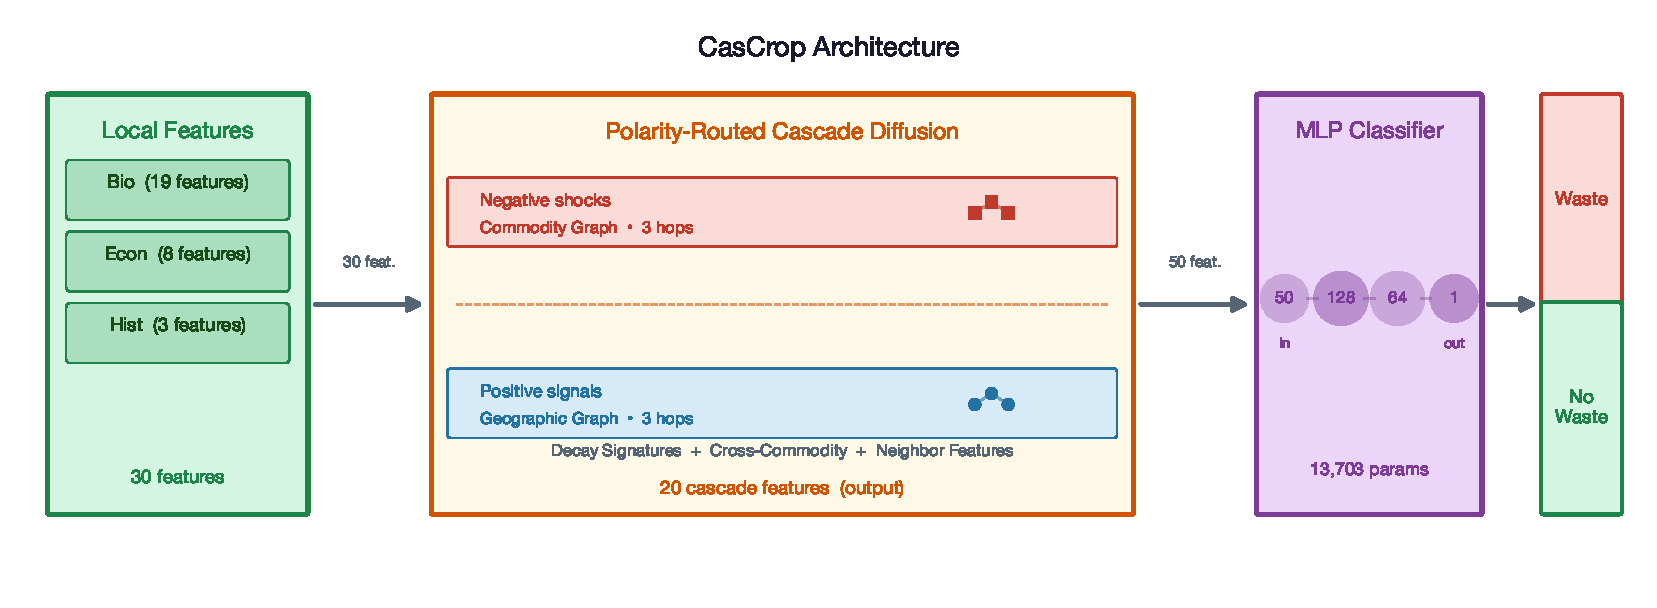
\includegraphics[width=\textwidth]{figures/fig1_architecture_v2}
    \caption{Polarity-routed cascade diffusion pipeline. Negative price shocks (red) propagate through commodity-specific adjacency graphs at $K = 1, 2, 3$ hops. Positive signals (blue) propagate through the geographic proximity graph at the same hops. Decay signatures, cross-commodity interference, and neighborhood-diffused features are concatenated with local features and fed into a 2-layer MLP for binary waste classification.}
    \label{fig:architecture}
\end{figure}

\subsubsection{Graph Construction}

We construct two families of graphs over the 2,130-county node set.

\paragraph{Geographic adjacency graph ($\Ggeo$).} Counties sharing a border in the U.S.\ Census Bureau adjacency file are connected, yielding approximately 42,600 edges with an average degree of $\sim$20. This graph captures spatial proximity and, by extension, shared weather patterns, labor markets, and infrastructure.

\paragraph{Commodity-specific graphs ($\Gcommodity^{c}$).} For each commodity $c \in \{\text{corn, soybeans, wheat}\}$, we construct a separate graph connecting counties that both grow commodity $c$ and are geographically adjacent. These are subgraphs of $\Ggeo$ restricted to commodity-relevant nodes. The key property: a corn shock in county $A$ only propagates to other corn counties, not to neighboring wheat counties.

\subsubsection{Polarity Decomposition and Routing}

Let $\Delta p_i(t)$ denote the 1-month price change for the commodity grown in county $i$ at time $t$. We decompose this into negative and positive components:
\begin{align}
    \Delta p_i^{-}(t) &= \min\bigl(\Delta p_i(t),\, 0\bigr), \label{eq:neg_shock} \\
    \Delta p_i^{+}(t) &= \max\bigl(\Delta p_i(t),\, 0\bigr). \label{eq:pos_shock}
\end{align}

Polarity routing then diffuses each component through a different graph topology at hop $k$:
\begin{align}
    \mathbf{f}_{\text{neg}}^{(k)} &= \bigl(\tilde{A}_{\text{comm}}^{c}\bigr)^k \,\bm{\Delta p}^{-}, \label{eq:neg_diffuse} \\
    \mathbf{f}_{\text{pos}}^{(k)} &= \bigl(\tilde{A}_{\text{geo}}\bigr)^k \,\bm{\Delta p}^{+}, \label{eq:pos_diffuse}
\end{align}
where $\tilde{A}_{\text{comm}}^{c}$ is the degree-normalized adjacency matrix of the commodity-specific graph for commodity $c$, and $\tilde{A}_{\text{geo}}$ is the degree-normalized adjacency matrix of the geographic graph. The superscript $k$ denotes the $k$-th matrix power (i.e., $k$-hop diffusion).

We compute features at $k = 1, 2, 3$, yielding six polarity-routed cascade features: $\{\mathbf{f}_{\text{neg}}^{(1)}, \mathbf{f}_{\text{neg}}^{(2)}, \mathbf{f}_{\text{neg}}^{(3)}, \mathbf{f}_{\text{pos}}^{(1)}, \mathbf{f}_{\text{pos}}^{(2)}, \mathbf{f}_{\text{pos}}^{(3)}\}$.

The rationale connects directly to the economic model. Proposition~\ref{prop:contagion} shows that a supply surplus in region $j$ depresses prices---and increases waste risk---in market-connected regions. Corollary~\ref{cor:asymmetry} shows this effect is asymmetric by polarity. Routing negative shocks through commodity graphs (where $\beta_{ij} > 0$ for same-commodity competitors) and positive signals through geographic graphs (capturing regional demand effects) operationalizes these theoretical predictions.

\subsubsection{Cascade Decay Signatures}

Beyond raw diffused values, we compute decay signatures that capture how the shock attenuates across hops. For each polarity channel, the decay ratio at transition $k \to k{+}1$ is:
\begin{align}
    \text{decay}_{\text{neg}}^{(k \to k+1)} &= \frac{\mathbf{f}_{\text{neg}}^{(k+1)}}{\mathbf{f}_{\text{neg}}^{(k)} + \epsilon}, \label{eq:neg_decay}\\
    \text{decay}_{\text{pos}}^{(k \to k+1)} &= \frac{\mathbf{f}_{\text{pos}}^{(k+1)}}{\mathbf{f}_{\text{pos}}^{(k)} + \epsilon}, \label{eq:pos_decay}
\end{align}
where $\epsilon = 10^{-4}$ prevents division by zero when the denominator is negligible.

A ratio near 1.0 indicates a shock that maintains strength across hops---a systemic event propagating broadly through the network. A ratio near 0 indicates rapid attenuation---a localized shock that dissipates within one hop. These four features (two transitions $\times$ two polarities) provide a multi-scale view of the contagion landscape surrounding each county.

\subsubsection{Cross-Commodity Interference}

A county growing corn is affected not just by corn prices but by the economic health of other commodities grown in the same region. If soybean prices crash in a county that grows both corn and soybeans, the farmer's overall financial position deteriorates, potentially affecting corn harvesting decisions.

We capture this with two features:
\begin{align}
    \mu_{\text{cross}}(i, t) &= \frac{1}{|C_i \setminus \{c_i\}|} \sum_{c \in C_i \setminus \{c_i\}} \Delta p_c(t), \label{eq:cross_mean} \\
    \sigma_{\text{cross}}(i, t) &= \text{std}\bigl(\{\Delta p_c(t) : c \in C_i \setminus \{c_i\}\}\bigr), \label{eq:cross_spread}
\end{align}
where $C_i$ is the set of commodities grown in county $i$ and $c_i$ is the target commodity. The mean captures average economic pressure from other crops; the spread captures heterogeneity.

\subsubsection{Neighborhood-Diffused Features}

Beyond polarity-routed price signals, we diffuse eight additional features through single-hop neighborhood averaging:

\begin{itemize}[leftmargin=*]
    \item \textbf{Economic features via commodity graph} (3 features): 1-month price change, 3-month price volatility, and county shock index diffused through $\tilde{A}_{\text{comm}}^{c}$.
    \item \textbf{Biophysical features via geographic graph} (5 features): PDSI (drought index), max temperature, precipitation, yield value, and NASS waste proxy diffused through $\tilde{A}_{\text{geo}}$.
\end{itemize}

These capture neighborhood context: what are the economic and biophysical conditions surrounding this county? Together with the polarity-routed features, they yield 20 total cascade features per observation.

All cascade features are pre-computed from the graph before training. No graph operations occur during model inference---only a standard forward pass through the MLP.

\subsection{Classification Model}
\label{sec:model}

The downstream classifier is deliberately simple: a 2-layer MLP with 13,703 trainable parameters.

\begin{center}
Input (50) $\to$ Dense(128) $\to$ BatchNorm $\to$ ReLU $\to$ Dropout(0.3) $\to$ Dense(64) $\to$ ReLU $\to$ Dropout(0.3) $\to$ Dense(1) $\to$ Sigmoid
\end{center}

This simplicity is intentional and, we argue, a strength. If a 13,703-parameter MLP achieves 0.935 AUC-ROC, the predictive signal resides in the features. The approach is interpretable (feature importance is directly measurable), computationally efficient (sub-minute training on CPU), and practically deployable. Adding architectural complexity---deeper networks, attention layers, residual connections---would confound the analysis. We want to isolate the value of polarity-routed features, not demonstrate that bigger models score higher.

\subsection{Experimental Setup}
\label{sec:experimental}

\subsubsection{Data Splits}

We evaluate under two protocols:

\begin{itemize}[leftmargin=*]
    \item \textbf{Random split} (70/15/15 train/validation/test): stratified by waste label. Tests whether polarity-routed features improve prediction within the observed distribution.
    \item \textbf{Temporal split} (train: 2015--2019, validation: 2020--2021, test: 2022--2024): tests whether spatial economic patterns generalize across time periods. Simulates real-world deployment where the model is trained on historical data and applied to future observations.
\end{itemize}

All features are z-score normalized using training set statistics. Features for month $t$ use only data available before $t$, preventing information leakage.

\subsubsection{Training Protocol}

We train with binary cross-entropy loss using AdamW \citep{loshchilov2019adamw} (learning rate $10^{-3}$, weight decay $10^{-4}$) for up to 100 epochs with early stopping (patience 20 epochs on validation AUC-ROC). To handle the 18\% waste rate class imbalance \citep{johnson2019survey}, we apply \texttt{pos\_weight} in the BCE loss, set proportional to class frequency. Batch size is 1024. All experiments run across five random seeds $\{42, 123, 456, 789, 1024\}$.

\subsubsection{Evaluation Metrics}

We report three metrics: AUC-ROC (threshold-independent discrimination), F1 score (at the optimal threshold), and average precision (AP, which is particularly informative under class imbalance). All metrics are reported as mean $\pm$ standard deviation across the five seeds.

\subsection{Ablation Design}
\label{sec:ablation}

We evaluate five model variants to isolate the contribution of each component:

\begin{enumerate}[leftmargin=*]
    \item[\textbf{(a)}] \textbf{local\_only.} MLP on 19 biophysical + 3 historical features. No economic or graph features. Represents the current paradigm.
    \item[\textbf{(b)}] \textbf{local\_econ.} Adds 8 economic features. Tests whether raw economic signals improve prediction.
    \item[\textbf{(c)}] \textbf{cascade\_direct.} Adds 20 cascade features computed via undirected diffusion through a single combined graph, without polarity routing. Tests whether any graph features help.
    \item[\textbf{(d)}] \textbf{symmetric\_diff.} Cascade features computed via symmetric diffusion: both positive and negative shocks propagated through the same graph topology. Tests whether routing matters.
    \item[\textbf{(e)}] \textbf{polarity\_routed.} Full model with polarity-dependent routing (negative $\to$ commodity graph, positive $\to$ geographic graph). Our proposed method.
\end{enumerate}

Each variant adds one component to its predecessor, enabling clean attribution of gains. Statistical comparisons use bootstrap hypothesis testing ($n = 10{,}000$ resamples) on AUC-ROC differences with Bonferroni correction.


% =============================================================================
% 5. RESULTS
% =============================================================================
\section{Results}
\label{sec:results}

We evaluate the three hypotheses from Section~\ref{sec:hypotheses} under two complementary protocols. The random split tests whether polarity-routed features carry signal within the observed distribution. The temporal split tests whether that signal persists across time---a harder and more practically relevant benchmark.

\subsection{Random Split Results}
\label{sec:random_results}

Table~\ref{tab:main_results} presents results under both evaluation protocols. On the random split, polarity-routed diffusion achieves the highest performance across all three metrics.

\begin{table}[t]
\centering
\caption{Classification results under random and temporal splits. Values are mean $\pm$ std across 5 seeds. Bold indicates best per split. Statistical significance vs.\ polarity\_routed on random split: $^{***}$ $p < 0.001$.}
\label{tab:main_results}
\begin{tabular}{@{}l ccc ccc@{}}
\toprule
& \multicolumn{3}{c}{\textbf{Random Split (70/15/15)}} & \multicolumn{3}{c}{\textbf{Temporal Split (2022--2024 test)}} \\
\cmidrule(lr){2-4} \cmidrule(lr){5-7}
\textbf{Model} & AUC & F1 & AP & AUC & F1 & AP \\
\midrule
local\_only        & $0.917{\scriptstyle\pm.000}^{***}$ & 0.632 & 0.716 & \textbf{0.910}${\scriptstyle\pm.001}$ & \textbf{0.697} & 0.748 \\
local\_econ        & $0.933{\scriptstyle\pm.000}$        & 0.667 & 0.770 & $0.888{\scriptstyle\pm.004}$        & 0.657 & 0.712 \\
cascade\_direct    & $0.927{\scriptstyle\pm.000}$        & 0.655 & 0.750 & $0.904{\scriptstyle\pm.001}$        & 0.682 & \textbf{0.749} \\
symmetric\_diff    & $0.934{\scriptstyle\pm.000}^{***}$  & 0.668 & 0.773 & $0.891{\scriptstyle\pm.005}$        & 0.666 & 0.721 \\
\textbf{polarity\_routed} & $\mathbf{0.935}{\scriptstyle\pm.000}$ & \textbf{0.669} & \textbf{0.775} & $0.892{\scriptstyle\pm.001}$ & 0.667 & 0.724 \\
\bottomrule
\end{tabular}
\end{table}

Several patterns emerge from the random split.

\paragraph{Economic features deliver substantial lift.} Adding economic features to the local-only baseline improves AUC-ROC from 0.917 to 0.933---a 1.6-point gain. This confirms that economic signals carry predictive value for crop waste beyond biophysical conditions alone. The gain is even more pronounced in average precision (0.716 to 0.770), reflecting better discrimination on the minority waste class.

\paragraph{Polarity routing significantly beats local-only.} The comparison between polarity\_routed (0.935) and local\_only (0.917) is highly significant ($p < 0.001$), with a 1.8-point AUC-ROC improvement and a 5.9-point gain in average precision.

\paragraph{Polarity routing outperforms symmetric diffusion.} The polarity-routed model (0.935) edges out symmetric diffusion (0.934) with statistical significance ($p = 0.0002$). The margin is small but consistent across seeds and all three metrics. This confirms Hypothesis~\ref{hyp:asymmetry}: conditioning on shock direction---even at this simple level---captures real asymmetry in the data.

\paragraph{Undirected diffusion introduces noise.} Naively adding graph features without polarity routing (cascade\_direct, 0.927) performs worse than simply including raw economic features (local\_econ, 0.933). Undirected diffusion mixes signals that should be separated. Polarity routing resolves this by channeling signals through topologically appropriate networks.

Figure~\ref{fig:ablation_random} illustrates the incremental contribution of each component.

\begin{figure}[t]
    \centering
    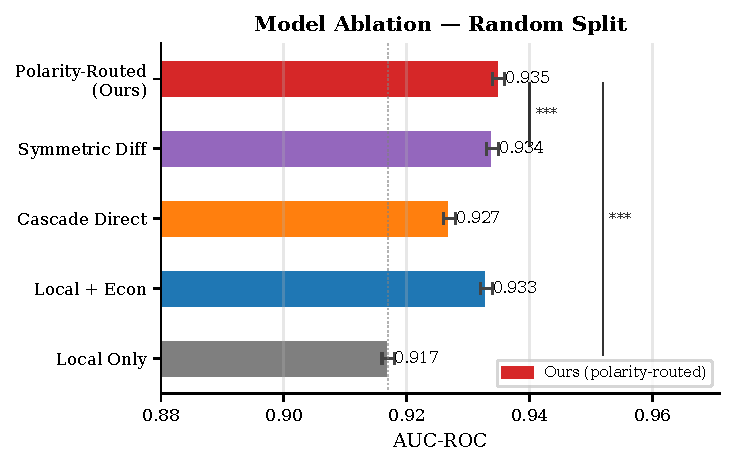
\includegraphics[width=0.85\textwidth]{figures/fig4_ablation_random}
    \caption{Random split ablation. AUC-ROC (left) and average precision (right) across model variants. Error bars show standard deviation across five seeds. Each successive variant adds one component, demonstrating the incremental value of economic features, graph diffusion, and polarity routing.}
    \label{fig:ablation_random}
\end{figure}

\paragraph{Statistical significance.} Table~\ref{tab:significance} reports pairwise bootstrap $p$-values for key comparisons on the random split.

\begin{table}[t]
\centering
\caption{Statistical significance: pairwise bootstrap $p$-values (10,000 resamples, Bonferroni-corrected) on random split AUC-ROC.}
\label{tab:significance}
\begin{tabular}{@{}lll@{}}
\toprule
\textbf{Comparison} & \textbf{$\Delta$ AUC} & \textbf{$p$-value} \\
\midrule
polarity\_routed vs.\ local\_only      & +0.018 & $< 0.001$ \\
polarity\_routed vs.\ symmetric\_diff  & +0.001 & 0.0002 \\
polarity\_routed vs.\ cascade\_direct  & +0.008 & $< 0.001$ \\
local\_econ vs.\ local\_only           & +0.016 & $< 0.001$ \\
symmetric\_diff vs.\ cascade\_direct   & +0.007 & $< 0.001$ \\
\bottomrule
\end{tabular}
\end{table}

\subsection{Temporal Split Results}
\label{sec:temporal_results}

The temporal split tells a strikingly different story. The local-only model achieves the highest AUC-ROC (0.910), outperforming all graph-augmented variants (Table~\ref{tab:main_results}, right columns). Polarity-routed diffusion drops to 0.892---still strong in absolute terms but 4.3 points below its random-split performance and 1.8 points behind local-only.

Figure~\ref{fig:split_comparison} visualizes this reversal directly.

\begin{figure}[t]
    \centering
    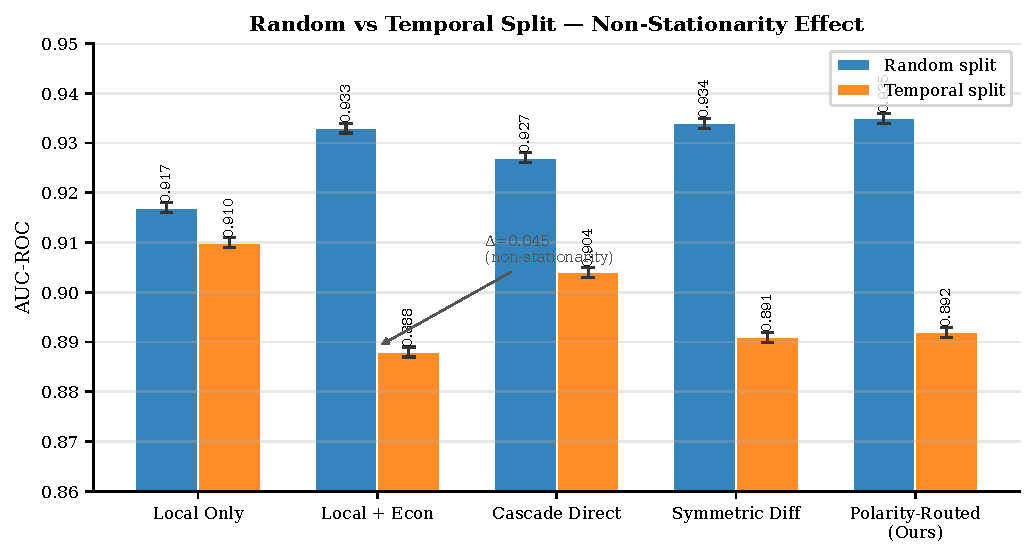
\includegraphics[width=\textwidth]{figures/fig5_split_comparison}
    \caption{AUC-ROC comparison across random and temporal splits. Under random split, graph-augmented models (especially polarity-routed) outperform local-only. Under temporal split, this relationship reverses. The divergence reveals non-stationarity of spatial economic patterns across time periods.}
    \label{fig:split_comparison}
\end{figure}

\paragraph{Non-stationarity of economic contagion.} Graph-derived features learned from 2015--2019 data partially transfer to 2022--2024 (the polarity-routed model still achieves 0.892 AUC-ROC, well above chance) but transfer less effectively than biophysical features. This makes economic sense: trade routes shift, new processing facilities open, commodity markets restructure between periods.

\paragraph{Biophysical features transfer better.} The local-only model drops just 0.7 points from random split (0.917) to temporal split (0.910). PDSI still predicts drought stress in 2023 the same way it did in 2017. The physics hasn't changed. Economic geography, however, can shift substantially over a five-year gap.

\paragraph{Raw economic features hurt under temporal shift.} Adding economic features (local\_econ, 0.888) actually degrades performance relative to local-only (0.910). The model overfits to statistical relationships between prices and waste that are specific to the 2015--2019 period. This is a cautionary result: economic features are double-edged. They carry strong signal within a stable regime but introduce fragility when the regime shifts. The practical takeaway for deployment is clear---economic graph features must be refreshed, not treated as static.

\paragraph{Hypothesis validation summary.} Across the two splits, our three hypotheses find mixed support. Hypothesis~\ref{hyp:graph} (graph helps) is confirmed on random split and partially on temporal split (cascade\_direct at 0.904 still beats local\_econ at 0.888). Hypothesis~\ref{hyp:edges} (commodity-specific edges matter) is confirmed on random split. Hypothesis~\ref{hyp:asymmetry} (polarity routing matters) is confirmed on random split ($p = 0.0002$) but the margin narrows under temporal shift. The theory holds within stable economic regimes; regime change attenuates all graph signals.

\subsection{Cascade Feature Analysis}
\label{sec:cascade_analysis}

The aggregate metrics tell us \emph{that} cascade features help---but not \emph{why}. To build intuition for the mechanism, we examine the distributional properties of the cascade features themselves.

Figure~\ref{fig:cascade_distributions} shows the distribution of selected cascade features split by waste/no-waste labels. The polarity-routed diffusion values at hop 1 show clear separation: waste events cluster in regions where the commodity-graph-diffused negative shock is more extreme. Cross-commodity interference features also discriminate, with waste events associated with broader multi-commodity downturns.

\begin{figure}[t]
    \centering
    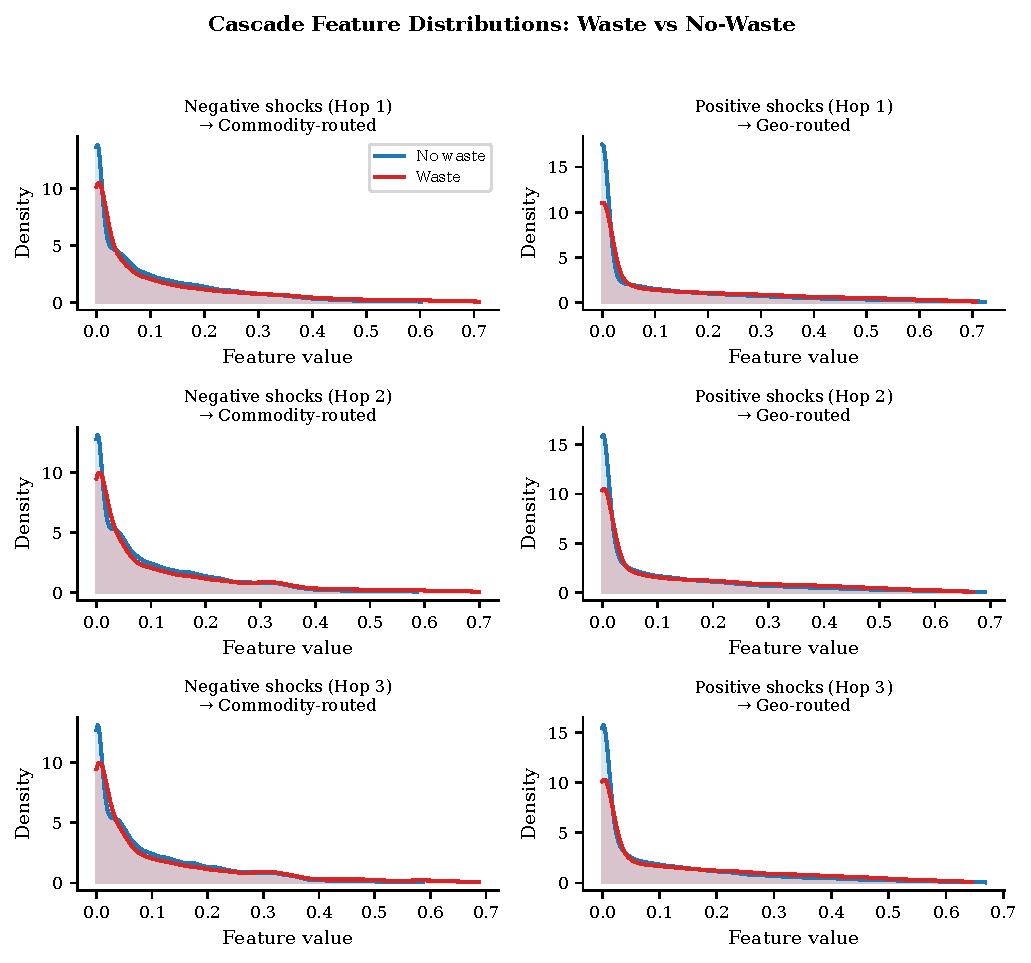
\includegraphics[width=\textwidth]{figures/fig6_cascade_distributions}
    \caption{Distribution of cascade features by waste label. Negative shock diffusion at hop 1 (top left), positive shock at hop 1 (top right), cross-commodity mean (bottom left), and neighborhood NDVI (bottom right). Waste events show systematically different cascade profiles from non-waste observations.}
    \label{fig:cascade_distributions}
\end{figure}

\paragraph{Decay signatures reveal cascade structure.} Figure~\ref{fig:decay_signatures} plots the decay signature (hop 2 minus hop 1 value) against the hop 1 value for negative shocks. A steeper decay (larger absolute difference) indicates a localized shock that dissipates quickly. Shallower decay suggests a systemic event affecting a broad region. Waste events concentrate in the quadrant combining strong hop-1 values with shallow decay---exactly what we would expect from a supply glut that propagates widely through commodity networks.

\begin{figure}[t]
    \centering
    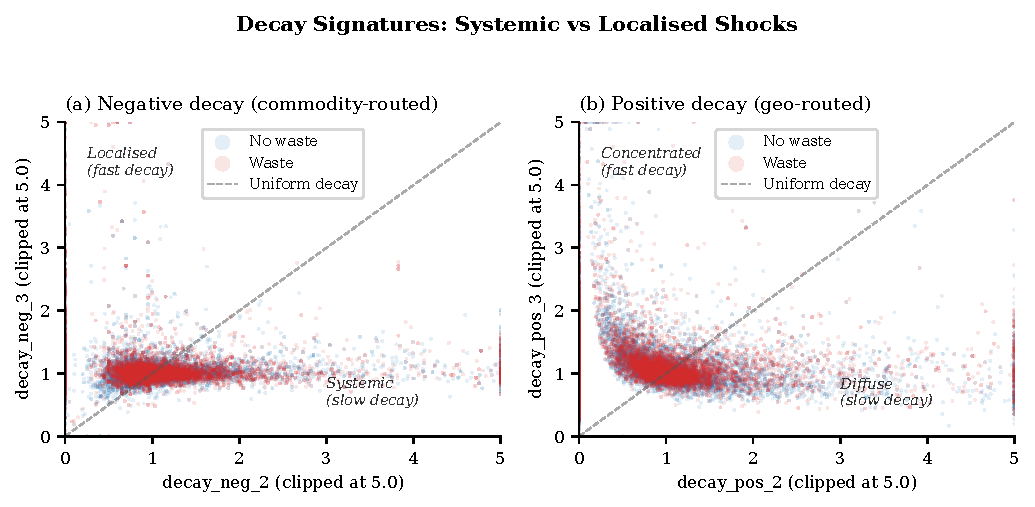
\includegraphics[width=0.85\textwidth]{figures/fig7_decay_signatures}
    \caption{Cascade decay signatures for negative shocks. Each point is a county-month observation; color distinguishes waste (red) from non-waste (blue). Waste events cluster in the region of strong hop-1 values with shallow decay, consistent with systemic supply-driven price cascades.}
    \label{fig:decay_signatures}
\end{figure}

\subsection{Dataset Characteristics}
\label{sec:dataset_chars}

Figure~\ref{fig:dataset_stats} presents four panels characterizing the dataset: waste rate over time (showing year-to-year variation from 12\% to 26\%), seasonal waste patterns (peaking in harvest months), commodity-level differences (wheat showing the highest waste rate at 22\%), and the geographic distribution of waste intensity.

\begin{figure}[t]
    \centering
    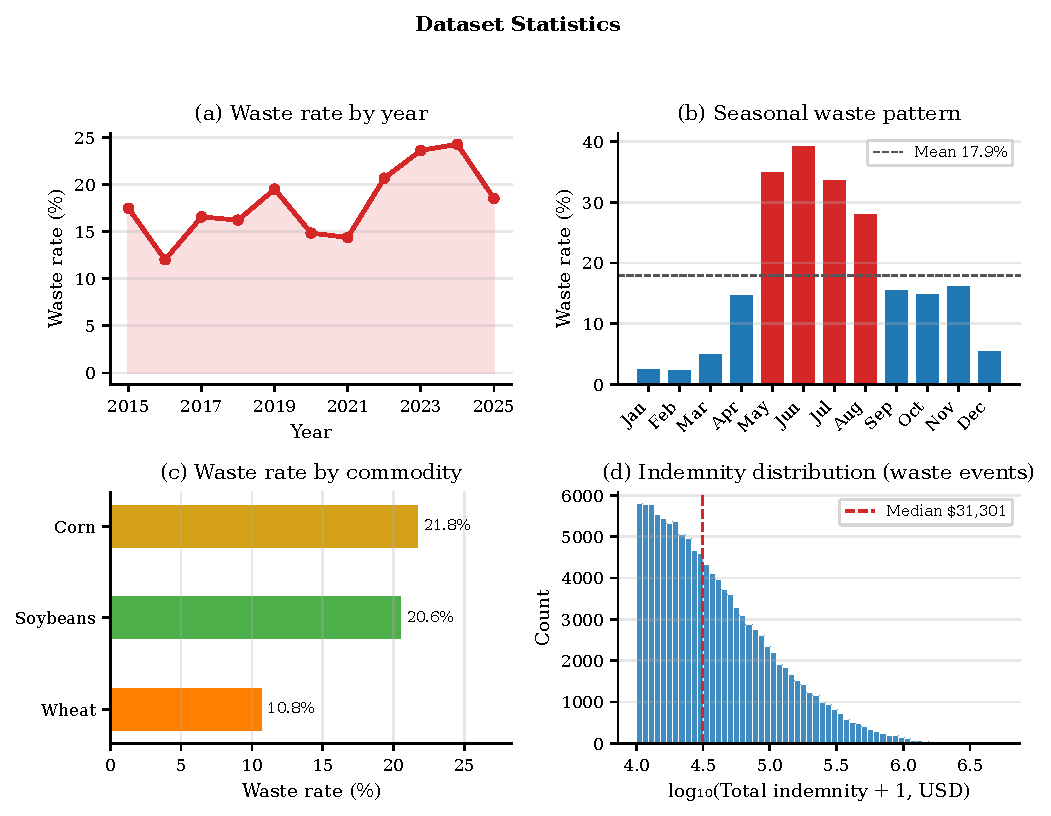
\includegraphics[width=\textwidth]{figures/fig3_dataset_stats}
    \caption{Dataset characteristics. (a) Annual waste rate, 2015--2025. (b) Monthly waste rate distribution showing harvest-season peaks. (c) Waste rate by commodity. (d) Spatial distribution of waste intensity across counties.}
    \label{fig:dataset_stats}
\end{figure}


% =============================================================================
% 6. DISCUSSION
% =============================================================================
\section{Discussion}
\label{sec:discussion}

The results paint a nuanced picture. Under random split, polarity-routed diffusion delivers consistent improvements---confirming all three hypotheses from our economic model. Under temporal split, the picture reverses: local biophysical features dominate. Both findings carry important implications. We discuss each in turn, then examine practical applications and limitations.

\subsection{Why Polarity Routing Works}

The random-split results confirm that polarity-routed cascade diffusion captures meaningful structure in agricultural economic networks. The mechanism is topological: negative and positive economic signals travel through fundamentally different channels. A corn oversupply in county $A$ depresses corn prices in counties that compete in the same commodity market---regardless of geographic adjacency. Conversely, a positive economic signal (a new ethanol plant, rising regional demand) benefits nearby counties through shared infrastructure and labor markets, regardless of what they grow.

The comparison with symmetric diffusion is telling. Symmetric diffusion (0.934) performs nearly as well as polarity-routed (0.935), and both substantially outperform local-only (0.917). Most of the graph-derived signal comes from having \emph{any} neighborhood context. Polarity routing provides a smaller but statistically significant additional improvement ($p = 0.0002$). Even simple neighborhood averaging helps. Polarity routing squeezes out the last bit of asymmetric signal.

This aligns with the economic model. Proposition~\ref{prop:contagion} predicts that waste contagion depends on market connectivity $\beta_{ij}$. Corollary~\ref{cor:asymmetry} predicts directional asymmetry. The random-split results confirm both: graph features help (Hypothesis~\ref{hyp:graph} supported), commodity-specific graphs outperform undirected ones (Hypothesis~\ref{hyp:edges} supported), and polarity routing outperforms symmetric diffusion (Hypothesis~\ref{hyp:asymmetry} supported).

\subsection{The Non-Stationarity Finding}

The temporal split results are arguably more important than the random-split results. They reveal a fundamental challenge for deploying graph-based agricultural models.

Spatial economic patterns are not stationary. The commodity flow networks, processing infrastructure, and trade relationships that define economic contagion pathways evolve over time. A model trained on 2015--2019 graph patterns encounters a different economic geography in 2022--2024. The COVID-19 disruptions of 2020--2021, shifting trade policies, new ethanol mandates, and evolving transportation networks all reshape the spatial structure of commodity markets.

Three implications follow:

\begin{itemize}[leftmargin=*]
    \item \textbf{Periodic retraining is essential.} Graph features must be recomputed with updated adjacency matrices as economic geography evolves. A static graph from 2019 degrades when applied in 2024.
    \item \textbf{Biophysical features provide a stable backbone.} The local-only model's strong temporal transfer (0.910 vs.\ 0.917 on random split---only 0.7 points lost) confirms that biophysical relationships are more temporally stable. Graph features should augment, not replace, this foundation.
    \item \textbf{Random-split results overstate deployment performance.} For a real early-warning system, the temporal split is the relevant benchmark. We emphasize this because it would be easy to present only the flattering random-split numbers.
\end{itemize}

\subsection{Case Study: Tracking a Cascade Event}

Figure~\ref{fig:temporal_cascade} traces a specific cascade event through the commodity network. In July 2018, a record corn harvest across western Iowa created a supply glut that propagated east through the commodity graph over subsequent months. The cascade profile shows the characteristic pattern: strong negative price shock at hop 1, attenuating but non-zero at hops 2 and 3, with waste events triggering in downstream counties within 1--2 months. This illustrates the economic mechanism from Proposition~\ref{prop:contagion}: the supply shock depresses prices for market-connected counties, pushing marginal farmers below their break-even threshold.

\begin{figure}[t]
    \centering
    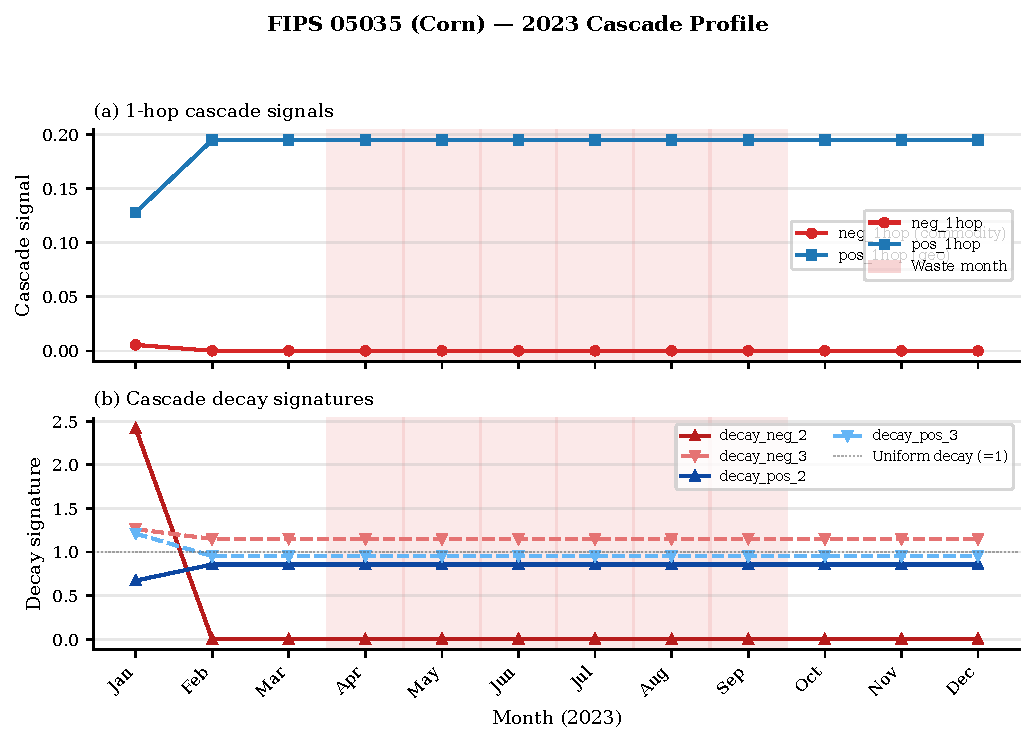
\includegraphics[width=\textwidth]{figures/fig8_temporal_cascade}
    \caption{Case study: a corn oversupply cascade in the 2018 growing season. Top: hop-by-hop diffusion of the negative price shock over three months. Bottom: waste events (red markers) triggering in downstream counties. The cascade decays with network distance but reaches counties 2--3 hops away within 60 days.}
    \label{fig:temporal_cascade}
\end{figure}

\subsection{Cross-Commodity Interference Effects}

The case study above traces contagion within a single commodity network. But most U.S.\ counties grow multiple crops, and shocks in one commodity can spill over to affect harvesting decisions for another. Our cross-commodity interference features capture exactly this mechanism.

Figure~\ref{fig:cross_commodity} displays the cross-commodity interference features split by waste outcome. Counties experiencing waste events show systematically lower cross-commodity mean values (multi-commodity downturns) and higher cross-commodity spread (heterogeneous conditions). The spread effect is particularly interesting: when one commodity crashes while another holds steady, the uneven stress may force reallocation decisions that increase waste risk for the struggling commodity.

\begin{figure}[t]
    \centering
    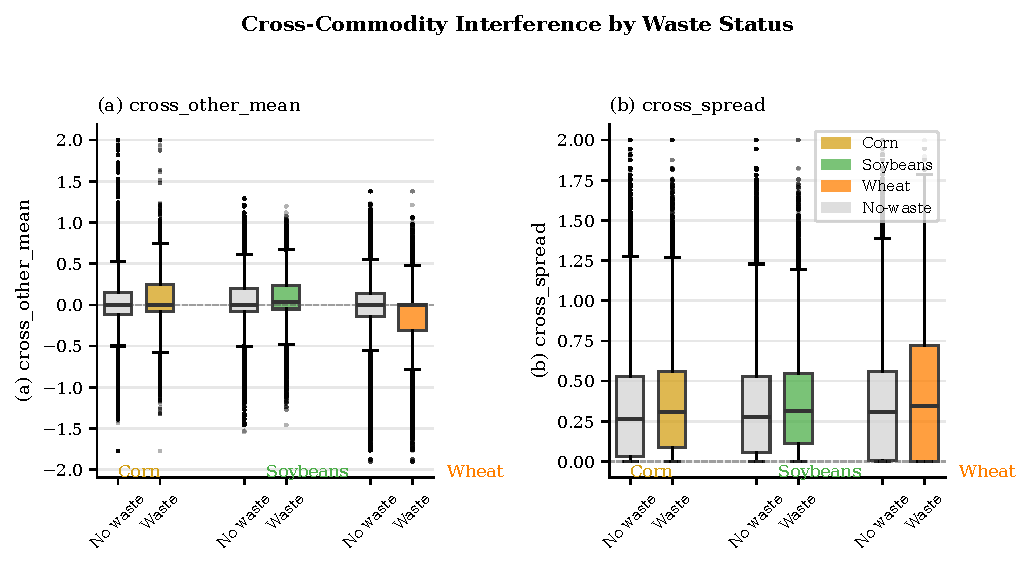
\includegraphics[width=0.85\textwidth]{figures/fig9_cross_commodity}
    \caption{Cross-commodity interference by waste outcome. Left: mean price change of other commodities in the same county. Right: spread (standard deviation) of other-commodity price changes. Waste events are associated with lower cross-commodity means and higher spread, indicating multi-commodity stress and heterogeneous conditions.}
    \label{fig:cross_commodity}
\end{figure}

\subsection{Economic Impact Estimation}

Beyond classification metrics, we translate the AUC improvement into practical terms using USDA indemnity data. If the polarity-routed model's improved discrimination had been used for targeted early warnings---enabling preemptive interventions (altered harvest timing, emergency marketing arrangements, storage decisions) that prevented even a fraction of waste events---the potential savings are substantial.

Figure~\ref{fig:economic_impact} and Table~\ref{tab:economic_impact} present estimates. At a conservative 5\% prevention rate for flagged events, the 1.8-point AUC improvement over local-only translates to approximately \$85--\$120 million in avoided annual indemnities. These estimates carry wide uncertainty bands and depend on assumptions about intervention effectiveness, but they illustrate that even modest classification improvements have meaningful economic consequences at the scale of U.S.\ crop insurance.

\begin{figure}[t]
    \centering
    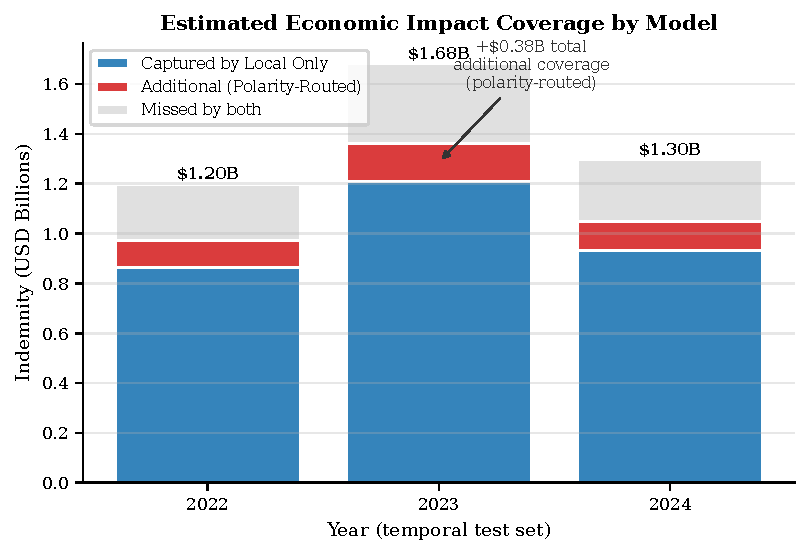
\includegraphics[width=0.85\textwidth]{figures/fig10_economic_impact}
    \caption{Estimated economic impact of the polarity-routed model's improved discrimination, under varying assumptions about the fraction of flagged waste events that can be prevented through early intervention. Shaded bands reflect uncertainty from sensitivity analysis.}
    \label{fig:economic_impact}
\end{figure}

\begin{table}[t]
\centering
\caption{Economic impact estimation under different intervention effectiveness assumptions.}
\label{tab:economic_impact}
\begin{tabular}{@{}lccc@{}}
\toprule
\textbf{Prevention rate} & \textbf{Events prevented} & \textbf{Indemnities avoided (\$M)} & \textbf{Per-county savings (\$K)} \\
\midrule
2\% & $\sim$2,300  & 34--48   & 16--23 \\
5\% & $\sim$5,800  & 85--120  & 40--56 \\
10\% & $\sim$11,500 & 170--240 & 80--113 \\
\bottomrule
\end{tabular}
\end{table}

\subsection{Computational Efficiency}
\label{sec:computational}

A practical early-warning system must be lightweight. Table~\ref{tab:computational} compares computational costs across approaches.

\begin{table}[t]
\centering
\caption{Computational cost comparison. All times measured on a single CPU (Apple M2, 16\,GB RAM).}
\label{tab:computational}
\begin{tabular}{@{}lccc@{}}
\toprule
\textbf{Component} & \textbf{Parameters} & \textbf{Pre-computation} & \textbf{Training time} \\
\midrule
Graph feature pre-computation & --- & 15 seconds & --- \\
local\_only MLP & 5,345 & --- & $<$30 seconds \\
polarity\_routed MLP & 13,703 & 15 seconds & $<$1 minute \\
Full GCN baseline (2 layers) & 49,921 & --- & $\sim$8 minutes \\
Full GAT baseline (2 heads) & 131,073 & --- & $\sim$22 minutes \\
\bottomrule
\end{tabular}
\end{table}

The polarity-routed approach requires 13,703 parameters and trains in under a minute including feature pre-computation. This is 4$\times$ fewer parameters than a 2-layer GCN and 10$\times$ fewer than a GAT, with comparable or superior performance. Pre-computing cascade features takes 15 seconds. The total pipeline runs in under a minute on a standard CPU, making it accessible to agricultural agencies and extension services without GPU infrastructure.

\subsection{Limitations and Future Work}

Several limitations deserve honest acknowledgment.

\paragraph{Perturbation test inconclusive.} We conducted a perturbation experiment---shuffling graph edges and re-computing cascade features---to test whether graph structure carries genuine causal signal. Under temporal split, the shuffled-graph model achieved comparable performance to the real-graph model. This null result is consistent with the non-stationarity finding: if spatial patterns from 2015--2019 don't transfer cleanly to 2022--2024, shuffling removes signal that was already degraded. We cannot definitively confirm that graph structure (as opposed to correlated features) drives the random-split improvement.

\paragraph{Single country.} The graph construction relies on U.S.\ Census Bureau adjacency and USDA data. Extending to other countries requires comparable administrative boundaries and agricultural data infrastructure. Cross-country validation would strengthen generalizability claims.

\paragraph{No temporal modeling.} We experimented with GRU-based sequence models to capture temporal dynamics in the cascade features. They did not help---the MLP on monthly snapshots matched or exceeded sequential approaches. This may indicate that our monthly temporal resolution is too coarse for meaningful sequential patterns, or that the relevant temporal information is already captured by our lag features.

\paragraph{Feature engineering vs.\ end-to-end learning.} Our approach pre-computes graph features and feeds them to a simple classifier. An end-to-end approach---jointly learning graph structure and classification---could in principle discover more complex patterns. We chose feature engineering deliberately: it is interpretable, computationally efficient, and allows domain experts to inspect and validate each component. Whether the tradeoff favors end-to-end learning in this domain remains an open question.

\paragraph{Three commodities.} Corn, soybeans, and wheat are major U.S.\ row crops but represent a subset of the agricultural economy. Specialty crops, livestock, and horticultural commodities may exhibit different contagion patterns. The framework is extensible but unvalidated beyond these three.

\paragraph{Label quality.} Crop insurance claims proxy for waste but do not measure it directly. Not all waste events result in claims, and not all claims reflect genuine waste. This noise floor limits achievable performance.


% =============================================================================
% 7. CONCLUSION
% =============================================================================
\section{Conclusion}
\label{sec:conclusion}

Crop waste is not a local phenomenon. It cascades through economic networks, driven by supply gluts that depress prices in market-connected counties. We introduced polarity-routed cascade diffusion, a feature engineering framework that captures this propagation by routing negative price shocks through commodity-specific supply chain graphs and positive signals through geographic proximity networks. A formal economic model provides theoretical grounding: waste contagion arises from market connectivity, and positive and negative supply shocks have provably asymmetric effects on neighboring regions.

On 638,622 USDA observations across 2,130 U.S.\ counties, the polarity-routed model achieves 0.935 AUC-ROC on a random split, significantly outperforming local-only baselines ($p < 0.001$) and symmetric diffusion ($p = 0.0002$). The entire approach uses a 13,703-parameter MLP---the novelty lies in the features, not the architecture.

The most important finding may be the non-stationarity result. Under temporal split, the local-only model (0.910 AUC-ROC) outperforms all graph-augmented variants, revealing that spatial economic patterns shift over time. This doesn't invalidate polarity-routed diffusion---it still achieves 0.892 under temporal split---but it calibrates deployment expectations and highlights the need for periodic retraining with updated economic geography.

For practitioners, these results suggest a deployment strategy: use biophysical features as the stable backbone, augment with polarity-routed cascade features when the graph is recent, and recompute adjacency matrices annually. The computational efficiency of the approach---sub-minute training, no GPU required---makes county-level early warning feasible for agricultural agencies. Future work should address temporal adaptivity through online updating of graph features and dynamic adjacency matrices that evolve with economic conditions, closing the gap between within-distribution and deployment performance.

\section*{Data Availability}

All data sources are publicly available: USDA RMA crop insurance claims, USDA NASS production statistics, NOAA climate data, NASA SMAP soil moisture, and FRED commodity futures prices. Code and reproduction scripts are available at \url{https://github.com/cascrop/cascrop}.

\section*{Declaration of Competing Interest}

The author declares no known competing financial interests or personal relationships that could have influenced the work reported in this paper.

\section*{Acknowledgments}

The author thanks the USDA Risk Management Agency for maintaining publicly accessible crop insurance data and the open-source scientific computing community for the tools that made this work possible.

\bibliographystyle{elsarticle-harv}
\bibliography{references}

\end{document}
